% +---------------------------------------------------------------+
% | Author :    Noémie Plancherel, HEIG-VD
% | Date :      18.04.2022
% +---------------------------------------------------------------+



\chapter{Étude de marché}
\label{ch:etude_marche}
Ce chapitre vise à étudier les différentes fonctionnalités offertes par les gestionnaires de mots de passe en les comparant entre plusieurs produits sélectionnés et en établissant un tableau afin d'avoir une meilleure vue d'ensemble.

Nous allons également analyser les différents prix des applications ainsi que présenter où en est le marché actuel afin d'étudier la popularité de ces dernières.

Pour l'étude de marché, les gestionnaires de mots de passe sélectionnés sont: \textit{LastPass}\footnote{\href{https://www.lastpass.com/}{https://www.lastpass.com/}}, \textit{Dashlane}\footnote{\href{https://www.dashlane.com/}{https://www.dashlane.com/}}, \textit{1Password}\footnote{\href{https://1password.com/}{https://1password.com/}}, \textit{KeePass}\footnote{\href{https://keepass.info/}{https://keepass.info/}}, \textit{Bitwarden}\footnote{\href{https://bitwarden.com/}{https://bitwarden.com/}}, \textit{NordPass}\footnote{\href{https://nordpass.com/}{https://nordpass.com/}}, \textit{Padloc}\footnote{\href{https://padloc.app/}{https://padloc.app/}}, \textit{Keeper}\footnote{\href{https://www.keepersecurity.com/}{https://www.keepersecurity.com/}}, \textit{Firefox}\footnote{\href{https://www.mozilla.org/fr/firefox/features/password-manager/}{https://www.mozilla.org/fr/firefox/features/password-manager/}}.

Ils ont été sélectionnés en se basant sur leur popularité sur le marché ainsi qu'à la suite de lecture d'articles concernant les meilleurs gestionnaires de mots de passe \cite{BPM22}\cite{gallagher19}\cite{MSPM22}\cite{PM22}. Les applications open-source ont été avantagées lors de leurs sélections.
\section{Fonctionnalités}
Ci-après, nous avons établi un tableau récapitulatif qui indique quels gestionnaires de mots de passe offre quelles fonctionnalités. Nous nous sommes basés sur les fonctionnalités citées dans le chapitre d'introduction \ref{intro}.

	\begin{figure}[H]
		\centering
		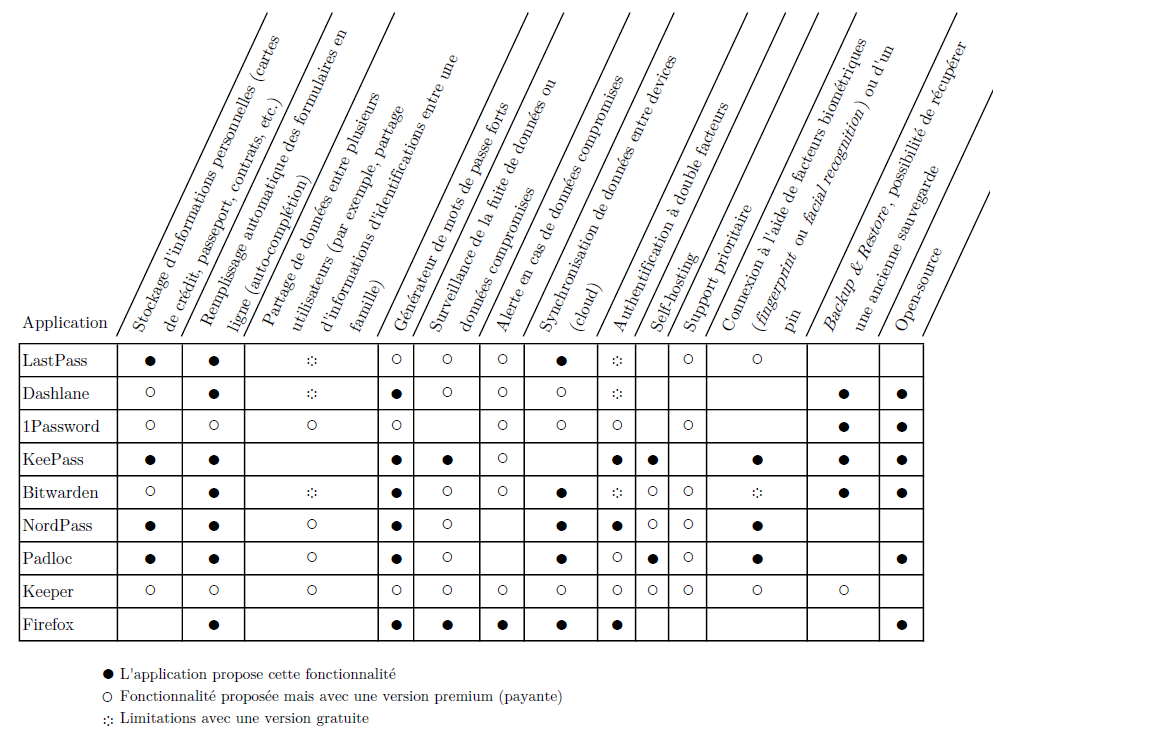
\includegraphics[width=18cm]{images/fonctionnalites.png}
		\captionof{table}{Fonctionnalités des candidats sélectionnés}
	\end{figure}


Sur tous les candidats sélectionnés, nous remarquons que la plupart offrent la majorité des fonctionnalités énumérées plus haut. Nous constatons que l'offre des constructeurs de gestionnaires de mots de passe est assez variée et répond à la demande des particuliers et des entreprises.

Pour KeePass, en général, il est nécessaire d'installer des plugins supplémentaires afin de profiter de toutes les fonctionnalités.

Par rapport aux restaurations de sauvegarde (\textit{Backup \& Recovery}), les gestionnaires sync-cloud vont automatiquement créer des backups sur les serveurs du constructeur toutes les nuits, donc la restauration se fait directement dans le gestionnaire. Pour Bitwarden, lorsque le gestionnaire est hébergé on-premise\footnote{Gestionnaire de mots de passe hébergé sur les serveurs de l'utilisateur, souvent utilisé dans des infrastructures d'entreprise}, il est nécessaire de créer ses propres procédures de sauvegardes. Etant donné que KeePass est uniquement en local, les sauvegardes doivent être faites manuellement et peuvent être importées sur l'application. Toutes ces solutions nécessitent le master password. Si ce dernier est oublié, il existe plusieurs solutions différentes en fonction des constructeurs (fonctionnalité pas disponible sur KeePass). 

La "sauvegarde" qui ne nécessite pas d'avoir son master password est l'exportation des données en fichier CSV, mais à moins de chiffrer le fichier, les données sont en claires ce qui n'est évidemment pas sécurisé et pas très recommandé.
\section{Plateformes}
Cette partie va permettre de visualiser sur quelles plateformes les gestionnaires de mots de passe sélectionnés sont supportés. \\
\begin{longtable}[H]{|c|c|c|c|c|c|c|}
	\hline
	Application & Windows & MacOS & Linux & Android & iOS & Navigateur  \\
	\hline
	LastPass & $\bullet$ & $\bullet$ & $\bullet$ & $\bullet$ & $\bullet$ &  $\bullet$\\
		\hline
	Dashlane & &  &  &&  & $\bullet$  \\
		\hline
	1Password & $\bullet$ & $\bullet$ & $\bullet$ & $\bullet$ & $\bullet$& \\
	\hline
	KeePass & $\bullet$ & $\circ$ & $\circ$  & $\circ$ & $\circ$ &  $\circ$  \\
		\hline
	Bitwarden & $\bullet$ & $\bullet$  & $\bullet$ & $\bullet$ & $\bullet$ & $\bullet$  \\
		\hline
	NordPass & $\bullet$ & $\bullet$ & $\bullet$  & $\bullet$ & $\bullet$ &  \\
		\hline
	Padloc & $\bullet$ & $\bullet$ & $\bullet$ & $\bullet$ & $\bullet$ & $\bullet$ \\
		\hline
	Keeper & $\bullet$ & $\bullet$ & $\bullet$ & $\bullet$ &$\bullet$ & $\bullet$ \\
		\hline
	Firefox & &  &  &&  & $\bullet$  \\
		\hline
	\caption{Plateformes supportées par les différentes applications}
\end{longtable}

$\bullet$ L'application est supportée sur ces plateformes \\
$\circ$  Des applications (ou des paquets) compatibles avec KeePass Password Safe non-officielles mais contribuées existent \\

Même si un gestionnaire supporte toutes les plateformes indiquées, il est nécessaire d'aller vérifier les conditions d'utilisation du système, c'est-à-dire les versions des plateformes afin de s'assurer que l'application fonctionnera quand même. 

Cependant, nous constatons que la majorité des applications sont disponibles sur les plateformes les plus courantes, et même si elles ne le sont pas, il y a souvent une solution non-officielle (notamment pour KeePass) ou via le navigateur qui existe.
\section{Prix}
Nous allons passer brièvement en revue les prix proposés par les gestionnaires de mots de passe. Chaque application propose leurs propres gammes de prix avec également des abonnements possibles pour les particuliers, familles ou entreprises. 
\subsection{Particuliers}
Pour la plupart des applications, nous pouvons retrouver 3 gammes de prix; Gratuit, Premium, Famille. L'offre familiale va être plus chère car les gestionnaires de mots de passe sont conçus pour pouvoir avoir plusieurs gestionnaires chiffrés individuels. 

Les tarifs ci-dessous sont exprimés en mensualités et en USD. \\
\begin{longtable}[h]{|c|c|c|c|}
		\hline
	Application & Gratuit & Premium & Famille \\
		\hline
	LastPass & \$0 & \$3 & \$4  \\
		\hline
	Dashlane & \$0 & \$3.99 & \$5.99 \\
		\hline
	1Password & non & \$2.99 & \$4.99  \\
		\hline
	KeePass & \$0 & non & non   \\
		\hline
	Bitwarden & \$0 & <\$1 & \$3.33   \\
		\hline
	NordPass & \$0 & \$1.84 & \$4.99  \\
	\hline
	Padloc & \$0 & \$3.49 & \$5.95    \\
	\hline
	Keeper & non & \$2.92 & \$6.25  \\
	\hline
	Firefox & non & non & non  \\
	\hline
\caption{Tarifs pour particuliers}
\end{longtable}
\subsection{Entreprises}
Les entreprises ont quant à elle des prix différents dû à leurs besoins spécifiques où ils pourraient avoir besoin d'un devis personnel afin de choisir l'abonnement qui convient au mieux à leur infrastructure. Il existe plusieurs catégories qui sont en fonction du nombre d'employés et également par rapport aux fonctionnalités souhaitées. 

Chaque prix est indiqué en mensualités, en USD et par employé.
\begin{longtable}[h]{|c|c|c|}
	\hline
	Application & Team & Business \\
	\hline
	LastPass & \$4 & \$6  \\
	\hline
	Dashlane & \$5 & \$8 \\
	\hline
	1Password & non  & \$7.99  \\
	\hline
	KeePass & non & non \\
	\hline
	Bitwarden & \$3 & \$5  \\
	\hline
	NordPass & non & \$3.50\footnote{Il y a la possibilité d'établir un devis en fonction des besoins spécifiques de l'entreprise \label{premium}} \\
	\hline
	Padloc & \$3.49 & \$6.99\footnote{voir \ref{premium}} \\
	\hline
	Keeper & non & \$3.75\footnote{voir \ref{premium}}  \\
	\hline
	Firefox & non & non \\
    \hline
	\caption{Tarifs pour les entreprises}
\end{longtable}

\section{Récapitualtif de l'étude}
Nous allons résumer toutes les informations que nous avons recueillies dans ce chapitre-ci; au final, nous constatons que les gestionnaires de mots de passe qui sont actuellement sur le marché (ici les plus populaires), sont assez complets au niveau des fonctionnalités proposées et ils sont adaptées pour tout type d'utilisation (personnelle, familiale ou professionnelle). Pour les gestionnaires payants, leurs prix sont assez abordables pour l'offre qu'ils proposent. Toutefois, même les gestionnaires en version gratuite, convient tout à fait à une utilisation quotidienne.

Au niveau des applications comparées, toutes ont leurs points positifs et leurs points négatifs (l'aspect sécuritaire sera discuté dans le chapitre \hyperref[ch:etude_secu]{\textit{étude sécuritaire}}). 

\textbf{LastPass} propose une version gratuite avec les fonctionnalités classiques que l'on attend d'un gestionnaire de mot de passe. La limite est que l'application n'est accessible que depuis un seul type d'appareil, ils font la différence entre ordinateur (fixe et portable) et appareil mobile (téléphone, montre, tablette). La version payante offre le MFA ainsi qu'un dashboard (avec les alertes de sécurité et la surveillance sur les données compromises), ce qui est une fonctionnalité intéressante.

La version gratuite de \textbf{DashLane} propose un stockage jusqu'à 50 mots de passe, ce qui est au final assez limtité mais il offre le 2FA ainsi que le partage sécurisé (jusqu'à 5 comptes). La version premium, permet l'utilisation d'un VPN ainsi qu'une synchronisation sur plusieurs appareils.

\textbf{1Password} est totalement payant mais est l'un des gestionnaires de mots de passe le plus populaire sur le marché.

\textbf{KeePass} est une application gratuite et open-source. Il propose une grande sélection de plugins assez utiles et variés, ce qui permet une grande offre, en plus d'être complètement gratuite.

\textbf{bitwarden} propose une version gratuite étonnement très complète avec un stockage illimité de mots de passe et un nombre illimité d'appareils. La version premium offre un 2FA avancé (notamment la connexion à l'aide d'une Yubikey) ainsi que des rapports de sécurité.

\textbf{NordPass} propose également une version gratuite complète qui permet le MFA ou encore la synchronisation entre plusieurs appareils, ce qui est très utile. Le premium propose l'aspect sécuritaire en plus. Cependant, c'est la solution gratuite la meilleure de tous les candidats sélectionnés.

\textbf{Padloc} n'est pas un gestionnaire très populaire mais il l'avantage d'être open-source et d'être disponible sur Github\footnote{\href{https://github.com/padloc/padloc}{https://github.com/padloc/padloc}}. La version gratuite n'offre pas beaucoup de fonctionnalités mais il y a la possibilité de stocker un nombre illimité de secrets et d'y connecter un nombre illimité d'appareils. De plus, il est multi-plateformes.

\textbf{Keeper} est complètement payant mais a une offre très complète et est particulièrement bien adapté pour les entreprises.

Finalement, le gestionnaire de mots de passe proposé par \textbf{Firefox} est directement inclus avec le navigateur, ainsi ses fonctionnalités proposées sont assez basiques et pas très poussées, mais il propose les fonctionnalités attendues d'un gestionnaire, c'est-à-dire enregistrement, génération et synchronisation de mots de passe.
